% Required packages:
% \usepackage{booktabs}
% \usepackage{graphicx}
% \usepackage{multirow}
% \usepackage{amsmath}

\subsection{Experimental Results and Analysis}

We evaluate SageFlow on five complementary closed-loop scenarios
constructed from nuPlan maps: (a) single-agent straight-road planning,
(b) a curved-road interaction, (c) dense multi-vehicle interaction,
(d) pedestrian crossing, and (e) a roundabout turn with two
interacting vehicles.
The scenarios jointly cover
free-space interaction, static and dynamic constraints, vulnerable road
users, and dense multi-agent traffic.  We first isolate the generator
used by SageFlow, comparing the original Flow Matching (FM) transport
field with the Rectified Flow (RF) field.  We then compare SageFlow with
three representative planner families: the learning-based Flow Planner,
the rule-based PDM planner, and the optimization-based MPC-CBF planner.

\begin{figure*}[t]
    \centering
    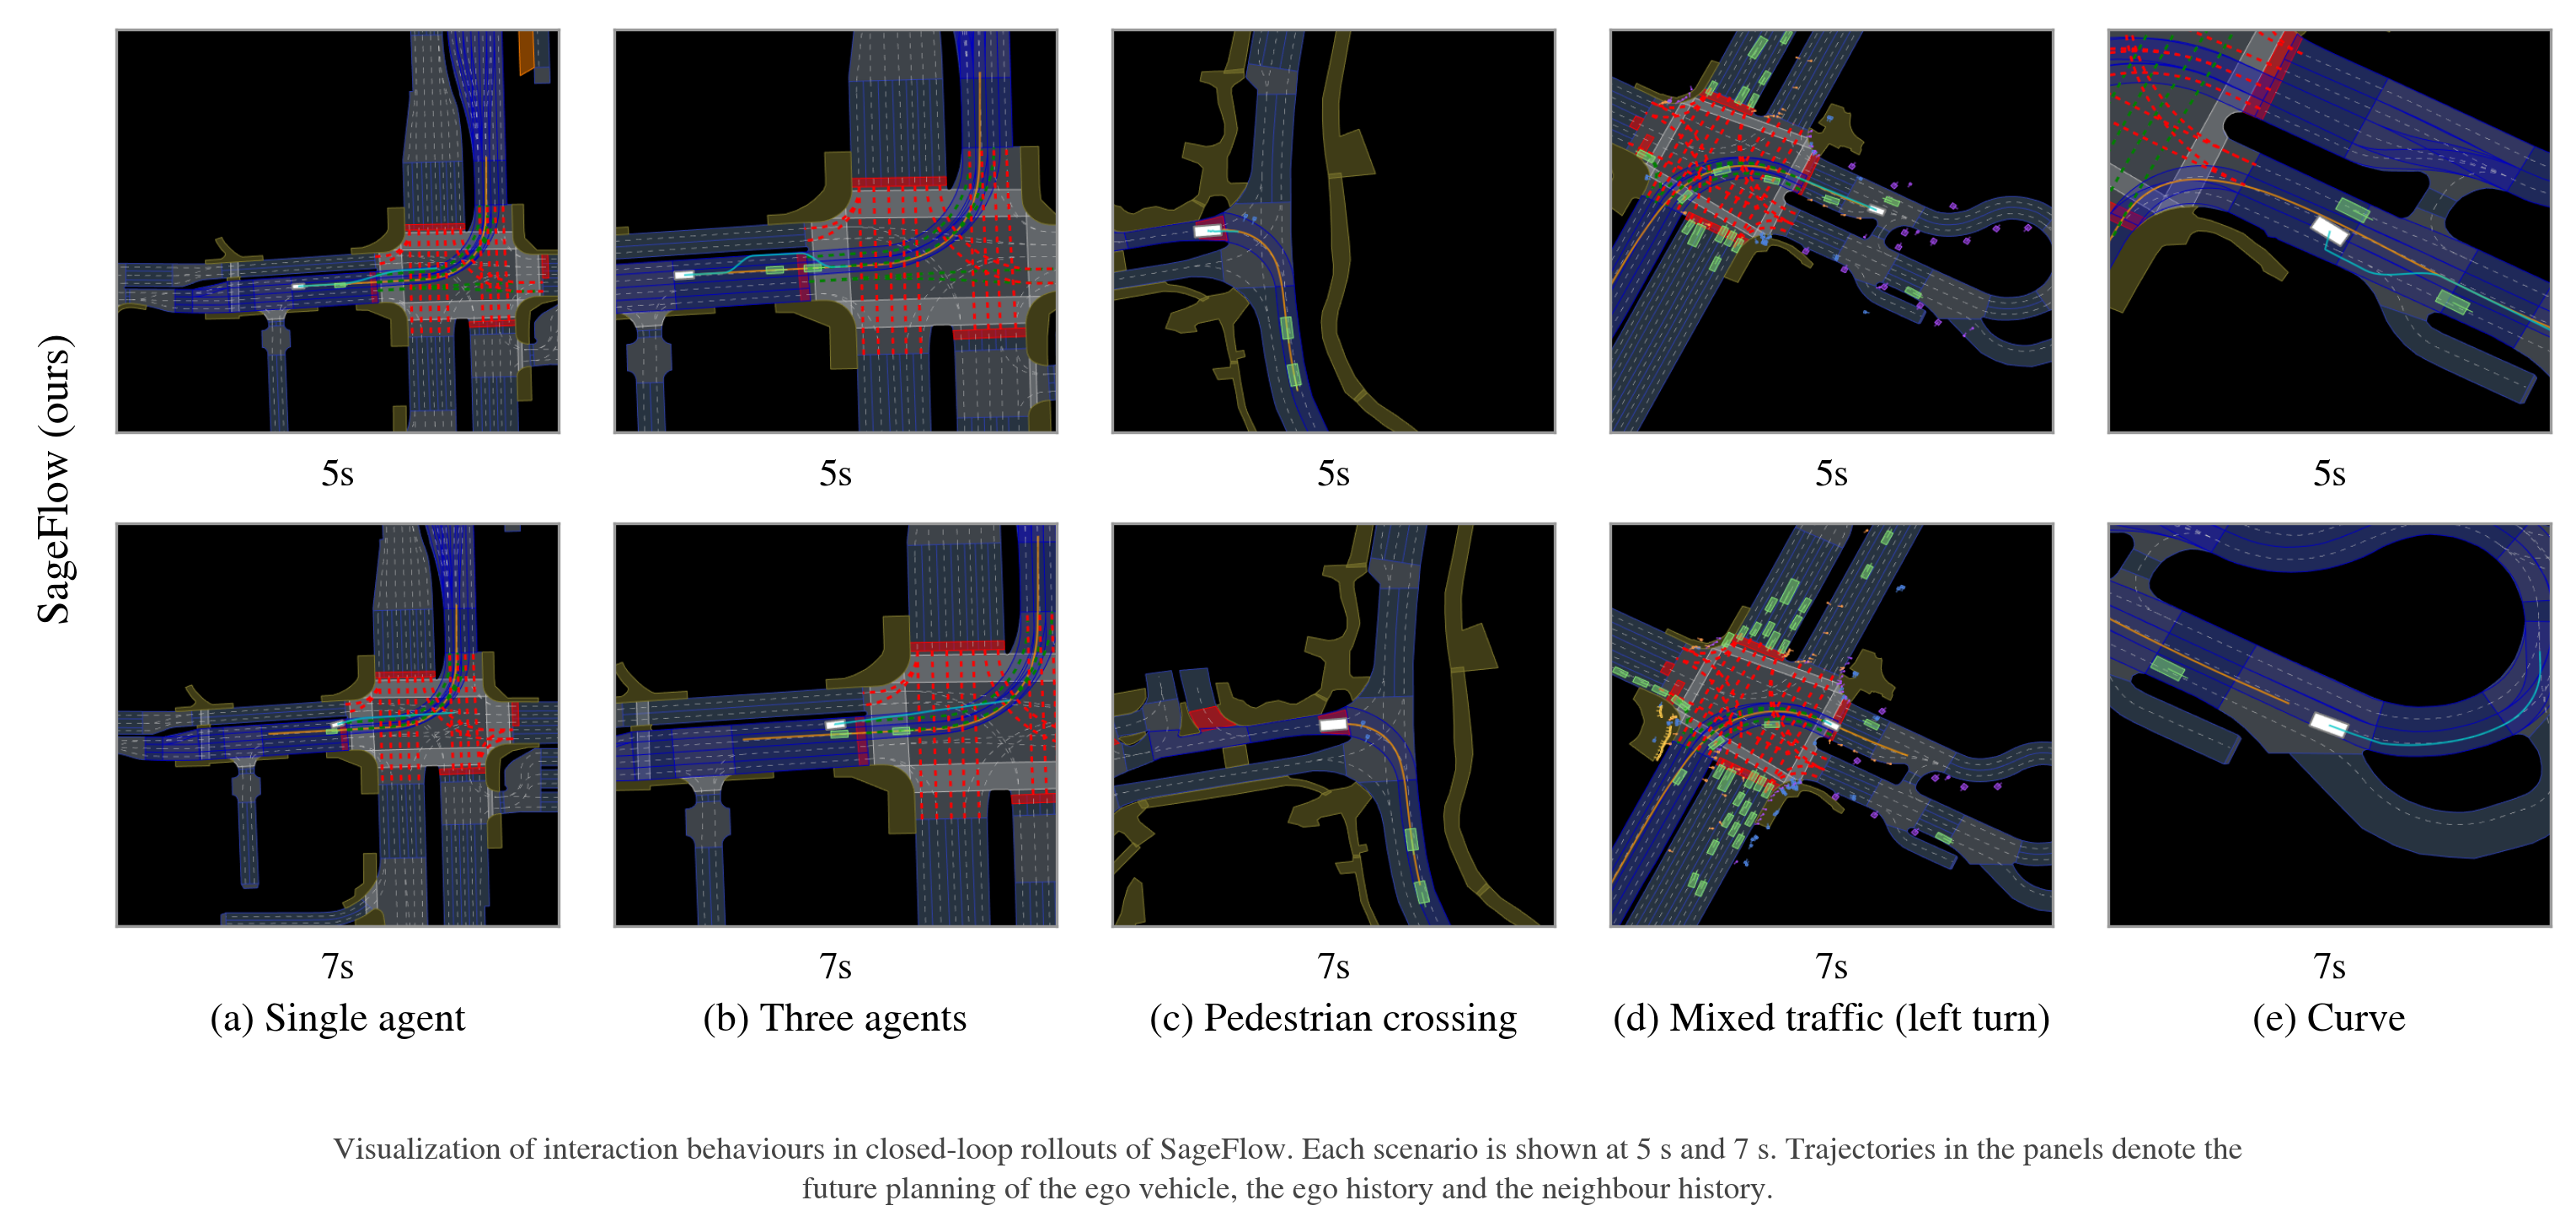
\includegraphics[width=0.98\textwidth]
    {fig_sageflow_scenarios_5s_7s_grid_white.png}
    \caption{Closed-loop rollouts of SageFlow in five nuPlan-map scenarios
    at 5\,s and 7\,s: (a) single-agent planning, (b) curved-road
    interaction, (c) dense multi-vehicle interaction, (d) pedestrian
    crossing, and (e) roundabout-turn interaction.  SageFlow preserves the
    interaction geometry while satisfying collision and direction
    constraints; the roundabout-turn case reveals the remaining
    drivable-area limitation.}
    \label{fig:sageflow_scenarios}
\end{figure*}

\paragraph{Scenario-level results.}
Table~\ref{tab:sageflow_generator_ablation} reports the five-scenario
results of SageFlow with the FM generator and with the RF generator.
All results use the same controller, canonical representation, CBF
projection, and execution pipeline.  The RF variant uses two ODE
segments, which we denote as RF-2.  This controlled comparison isolates
the effect of replacing the learned transport field.

Both generators remain collision-free and satisfy driving-direction
compliance in the five reported runs.  The roundabout-turn case is
the only exception to drivable-area compliance: both generators
complete the route safely but leave the drivable area during the
turn.  The main
difference is behavioral.  FM is more conservative on the straight-road
overtaking case and on the pedestrian-crossing case, where it favors
following or yielding over aggressive progress.  RF-2 clearly improves
route progress in the curved and dense multi-vehicle scenes: it reaches
\(0.893\) route ratio in the curve scenario and \(1.000\) in the
multi-vehicle scenario.  The corresponding composite scores are
\(0.800\) and \(0.894\), respectively.  Over the five scenarios, the
average planning latency of RF-2 is \(64.8\)\,ms, substantially below
the \(150.1\)\,ms of the FM configuration.  The turn case exposes the
remaining map-compliance limitation and motivates separating
collision safety from composite-score performance.

\begin{table*}[t]
    \centering
    \small
    \caption{Scenario-wise generator ablation of SageFlow.  FM denotes
    the original Flow Matching transport field, and RF-2 denotes the
    Rectified Flow field with two ODE segments.  CF indicates whether
    no ego-at-fault collision occurred.  Latency is the mean
    closed-loop planner computation time per iteration.  A zero score
    indicates failure of at least one multiplicative constraint term
    and does not necessarily indicate a collision.}
    \label{tab:sageflow_generator_ablation}
    \begin{tabular}{llccccccc}
        \toprule
        Generator & Scenario & Route \(\uparrow\) & Progress (m) \(\uparrow\)
        & CF \(\uparrow\) & Drivable \(\uparrow\) & Comfort \(\uparrow\)
        & Latency (ms) \(\downarrow\) & Score \(\uparrow\) \\
        \midrule
        \multirow{5}{*}{FM}
        & Straight      & 0.671 & 82.17  & Yes & 1.000 & No  & 94.3  & 0.643 \\
        & Curve         & 0.777 & 80.47  & Yes & 1.000 & Yes & 194.3 & 0.913 \\
        & Multi-vehicle & 0.841 & 102.97 & Yes & 1.000 & No  & 183.0 & 0.804 \\
        & Pedestrian    & 0.177 & 7.87   & Yes & 1.000 & Yes & 174.4 & 0.000 \\
        & Roundabout turn & 1.000 & 98.93 & Yes & 0.000 & No & 104.5 & 0.000 \\
        \midrule
        \multirow{5}{*}{RF-2}
        & Straight      & 0.290 & 35.47  & Yes & 1.000 & No  & 59.7  & 0.331 \\
        & Curve         & 0.893 & 92.50  & Yes & 1.000 & No  & 66.4  & 0.800 \\
        & Multi-vehicle & 1.000 & 128.00 & Yes & 1.000 & Yes & 50.5  & 0.894 \\
        & Pedestrian    & 0.166 & 7.40   & Yes & 1.000 & Yes & 85.9  & 0.000 \\
        & Roundabout turn & 1.000 & 98.93 & Yes & 0.000 & No & 61.6 & 0.000 \\
        \bottomrule
    \end{tabular}

    \vspace{0.5em}
    \parbox{0.96\textwidth}{\footnotesize
    The pedestrian case is a yielding behavior: the ego remains safe but
    does not complete the full route within the evaluation horizon.
    Therefore, its zero score should be interpreted as a conservative
    wait, not as a collision or constraint violation.  In the
    roundabout-turn case, both generators complete the route without
    an at-fault collision, but the trajectory violates the drivable
    area.  Since the nuPlan score multiplies its weighted metric
    average by the binary drivable-area term, this single violation
    sets the composite score to zero.  The RF-2 configuration is used
    consistently for the generator comparison.}
\end{table*}

\paragraph{Comparison with other planner types.}
Table~\ref{tab:planner_comparison} aggregates the five scenarios and
compares SageFlow with the learning-based Flow Planner, PDM, and
MPC-CBF.  PDM obtains the highest average composite score
(\(0.879\)), while MPC-CBF achieves the largest route progress and
performs well in the curved and multi-vehicle scenes.  Flow Planner is
the strongest learning-based baseline in the pedestrian-crossing
scenario, although it requires the second-largest planning latency.
SageFlow-RF-2 provides the lowest average planner
latency (\(64.8\)\,ms) among the compared methods while preserving
collision-free behavior in all five reported scenarios.

\begin{table}[t]
    \centering
    \small
    \setlength{\tabcolsep}{3pt}
    \caption{Aggregate comparison over the five closed-loop scenarios.
    Route is the mean expert-route progress ratio, CF is the number of
    collision-free scenarios out of five, and latency is measured on
    CPU.  The table reports controlled matched scenario runs and is
    not a statistical estimate over the full nuPlan benchmark.}
    \label{tab:planner_comparison}
    \resizebox{\columnwidth}{!}{
    \begin{tabular}{lccccccc}
        \toprule
        Method & Route \(\uparrow\) & Progress (m) \(\uparrow\)
        & CF \(\uparrow\) & Drivable \(\uparrow\) & Comfort \(\uparrow\)
        & Latency (ms) \(\downarrow\) & Score \(\uparrow\) \\
        \midrule
        Flow Planner       & 0.625 & 68.25  & 5/5 & 1.000 & 0.60 & 250.9 & 0.808 \\
        PDM                & 0.874 & 100.52 & 5/5 & 1.000 & 0.40 & 170.9 & 0.879 \\
        MPC-CBF            & 0.932 & 107.08 & 5/5 & 0.800 & 0.80 & 520.6 & 0.629 \\
        SageFlow-FM        & 0.693 & 74.48  & 5/5 & 0.800 & 0.40 & 150.1 & 0.472 \\
        SageFlow-RF-2      & 0.670 & 72.46  & 5/5 & 0.800 & 0.40 &  64.8 & 0.405 \\
        \bottomrule
    \end{tabular}}
\end{table}

\begin{table}[t]
    \centering
    \small
    \caption{Per-scenario composite score.  The density of interaction
    increases from the single-agent case to the roundabout-turn case.
    SageFlow-RF-2 is competitive in the curve and multi-vehicle
    scenarios, where interaction constraints are most pronounced.  A
    zero score indicates failure of at least one multiplicative
    constraint term, such as drivable-area compliance.}
    \label{tab:scenario_scores}
    \begin{tabular}{lccccc}
        \toprule
        Scenario & Flow Planner & PDM & MPC-CBF & SageFlow-FM & SageFlow-RF-2 \\
        \midrule
        Straight      & 0.898 & 1.000 & 0.625 & 0.643 & 0.331 \\
        Curve         & 0.679 & 0.792 & 0.967 & 0.913 & 0.800 \\
        Multi-vehicle & 0.780 & 0.730 & 0.867 & 0.804 & 0.894 \\
        Pedestrian    & 0.859 & 1.000 & 0.688 & 0.000 & 0.000 \\
        Roundabout turn & 0.821 & 0.875 & 0.000 & 0.000 & 0.000 \\
        \bottomrule
    \end{tabular}
\end{table}

The scenario-level comparison in Table~\ref{tab:scenario_scores}
shows that no single planner dominates all settings.  PDM performs
best in the straight and pedestrian scenarios, whereas MPC-CBF obtains
the highest score in the curve scenario.  SageFlow-RF-2 obtains the
highest score among the compared methods in the multi-vehicle scenario
(\(0.894\)), indicating that the rectified transport field is effective
when several dynamic obstacles must be resolved simultaneously.
In the curve scenario, SageFlow-FM obtains \(0.913\), showing that the
FM prior and the canonical CBF projection already provide a useful
interaction prior.  Replacing FM with RF-2 reduces latency while
retaining a competitive score.
In the roundabout-turn scenario, Flow Planner and PDM retain
drivable-area compliance and obtain composite scores of \(0.821\) and
\(0.875\), respectively.  MPC-CBF and both SageFlow generators complete
the route without an at-fault collision, but each trajectory violates
the drivable-area constraint during the turn.  Their zero composite
scores therefore indicate map-compliance failure, not collision
failure.

\paragraph{Behavioral analysis.}
Figure~\ref{fig:sageflow_scenarios} visualizes the resulting behavior.
In the single-agent case, SageFlow follows the lane geometry and keeps a
smooth trajectory.  In the dense multi-vehicle case, the ego trajectory bends
around the interacting vehicles instead of treating the obstacles as
independent geometric repairs.  In the pedestrian case, the ego yields
and preserves a safe stopping corridor before the crossing.
In the roundabout-turn case, the trajectory follows the turn and avoids
the interacting vehicles, but its lateral excursion remains a
drivable-area failure that is visible in the aggregate score.
These behaviors are consistent with the central design of SageFlow:
CBF acts as boundary-induced forcing, while the learned transport field
retains the multimodal motion prior.

\subsection{Ablation Study}

Table~\ref{tab:sageflow_generator_ablation} provides the generator-level
ablation.  FM and RF-2 use the same canonical frame, the same barrier
representation, and the same adaptive gate, so the difference measures
the effect of the learned transport parameterization.  The comparison
supports three observations.

\begin{enumerate}
    \item \textbf{Rectified Flow improves inference efficiency.}
    RF-2 reduces the mean planner latency from \(150.1\)\,ms to
    \(64.8\)\,ms over the five scenarios.

    \item \textbf{Rectified Flow improves dense interaction in the
    tested cases.}  The largest gains appear in the curve and
    multi-vehicle scenarios, where RF-2 reaches route ratios of
    \(0.893\) and \(1.000\), respectively.

    \item \textbf{Collision safety is preserved across generators.}
    Both generators produce collision-free trajectories in the five
    reported runs.  This indicates that the collision-safety mechanism is
    primarily enforced by the generation-time CBF projection rather
    than by the specific velocity-field parameterization.  Map
    compliance remains a separate limitation in the roundabout-turn
    scenario.
\end{enumerate}

For completeness, the component-level ablation should compare four
matched configurations: (i) the base generator without CBF,
(ii) the base generator with CBF, (iii) CBF with the adaptive
time/proximity gate disabled, and (iv) the full SageFlow model with the
canonical frame.  The current generator comparison already establishes
the RF component; the remaining component rows should be reported with
identical scenario tokens, horizon, and planner frequency before making
statistical claims.  In particular, the adaptive gate should be
analyzed separately from the CBF projection because it changes only the
scheduling of the correction, while the projection determines the
feasible correction direction.

\paragraph{Summary.}
The experiments show that SageFlow provides a collision-preserving
generative planning formulation across single-agent, multi-agent,
pedestrian, and turning scenarios.  RF-2 is the most efficient
generator configuration in the current study, while FM remains
competitive in the curve scenario.  The results also reveal the
expected trade-off: conservative yielding improves safety but reduces
route completion, whereas dense interaction benefits from the
rectified transport field.  These findings motivate reporting safety,
route progress, comfort, and computation time jointly rather than
using a single aggregate score.
